\documentclass[12pt]{article}
\usepackage[utf8]{inputenc}
\usepackage{natbib}
\usepackage{graphicx}
\usepackage{indentfirst}
\usepackage{amsfonts}
\usepackage{amsthm}
\usepackage{amsmath}
\usepackage[document]{ragged2e}
\usepackage{float}
\usepackage{listings}
\usepackage{pdfpages} 
\usepackage{caption}
\usepackage{subcaption}
\usepackage{verbatim}
\usepackage[margin=1.1in]{geometry}
\setlength{\parindent}{4em}
\setlength{\parskip}{1em}
\usepackage{caption}
\usepackage{subcaption}
\usepackage{biblatex}
\addbibresource{bibliography.bib}




\title{Bodyfat Dataset Analysis}


\author{ Thomas Grunauer, Jonathan Gorman, Seamus McCrave}
\date{December 2020}

\begin{document}

\maketitle

\section*{Introduction}

Body fat percentage -- like other measures of body composition -- seek to assess the health of an individual's body. Despite the importance of such measures, techniques to accomplish this are expensive and time consuming. The proposed data set, acquired from the DASL - Data and Story Library website, aims to find an alternative method of measuring body fat percentage using body dimensions. \cite{Tamhane}

\begin{figure}[h]
\centering
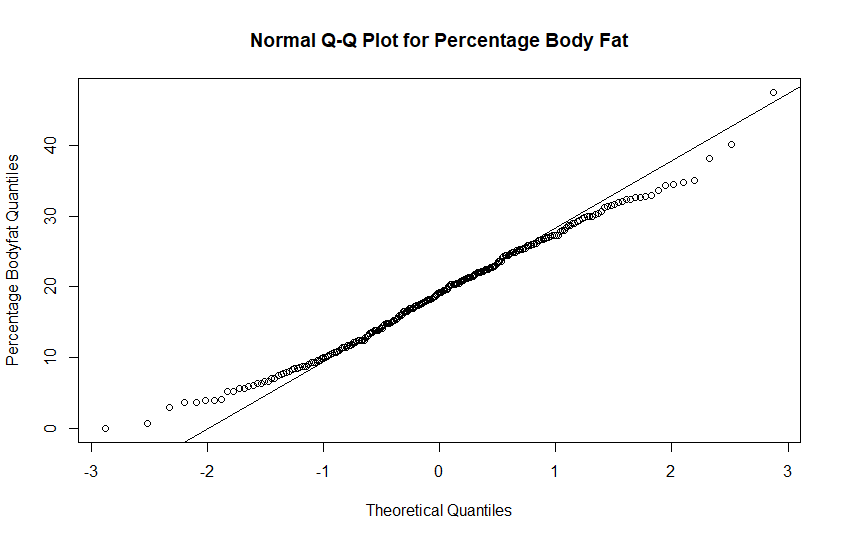
\includegraphics[width = 80mm]{qqplot_original_data_pctBF.PNG}
\caption{Normal plot of percentage body fat response variable}
\label{qqnorm_BF}
\end{figure}

The data set contains observations of 250 male subjects and measurements of the 16 variables outlined in table 1.\cite{Description} All except age is a continuous variable, and the division of age into broader categories is explained in the analysis of hypothesis 1. The primary goal of this analysis is to determine whether or not one can build a linear model based solely on easily measurable values. This excludes the body density as a predictive variable because it requires the subject to access a water displacement chamber. Furthermore, as explained in the hypothesis 2 section, body density is related to body fat percentage through Siri's Equation for body fat percentage\cite{sciencedirect}.

\begin{table}
\centering
\tabcolsep=0.11cm
\begin{tabular}{cc}
    \hline
    Variable Index & Variable Name \\
     \hline
     1  & Age  \\
     \hline
     2  & Weight \\
     \hline
     3  & Height \\
     \hline
     4  & Neck \\
     \hline
     5 & Chest \\
     \hline
     6 & Abdomen \\
     \hline
     7 & Hip \\
     \hline
     8 & Waist \\
     \hline
     9 & Thigh \\
     \hline
     10 & Knee \\
     \hline
     11 & Ankle \\
     \hline 
     12 & Bicep \\
     \hline
     13 & Forearm \\
     \hline 
     14 & Wrist \\
     \hline
     15 & Density \\
     \hline
     16 & \% Body Fat \\
     \hline
\end{tabular}
\caption{Variables measured for the subjects. Each variable is a measurement of the specified body dimension, except the age variable which is simply the participant's age.}
\end{table}

Each body dimension variable is measured as a circumference in centimeters except weight and height. To check that the percentage body fat response variable is normally distributed, one can use a normal plot and confirm the results with the Shapiro-Wilk test for normality.



In reference to figure 1, a majority of the data follows a normal trend, with some deviations at the tails of the distribution. These deviations are deemed unimportant by the Shapiro-Wilk test, which outputs a p-value of $0.1697$. The Shapiro-Wilk test's null hypothesis is that the data is normally distributed, thus, we cannot reject the null hypothesis that the data is normal even at a significance level of $\alpha = 0.1697$. The results of these tests imply that a transformation is not required to normalize the data for the response variable.

\section*{Hypothesis 1}
\begin{comment}
Upon first glance of the data set, there was a general trend that inferred that younger people had a lower body fat percentage while body fat percentage was slightly higher in older individuals. In treating age as a categorical variable,  51 distinct categories of age were left. To consolidate the number of categories, the data was broken down into two subsets. One which contained individuals under the age of 60, and the other which contained individuals aged 60 or older. For the purpose of simplicity, the latter group of individuals 60 years old or older will be referred to as senior citizens. We decided to make a side-by-side box plot to get a rough idea of the distribution of each of the groups. 
\end{comment}
Upon visual inspection, there was a noticeable difference between the body fat percentages of individuals under the age of 60 against those who were 60 years old or older.  Originally there were 51 distinct categories of age in the data set. To consolidate the number of categories, the data was broken down into two subsets.  Setting age to be either less than 60 or greater than/equal to 60, age is able to be considered a categorical variable which allows age to be used as a parameter for analysis. For the purpose of simplicity, the latter group of individuals 60 years old or older will be referred to as senior citizens \cite{paper}.  A side-by-side box plot is displayed below to aid as a visual in helping understand the distribution of each of the groups. 


\begin{figure}[h]
\centering
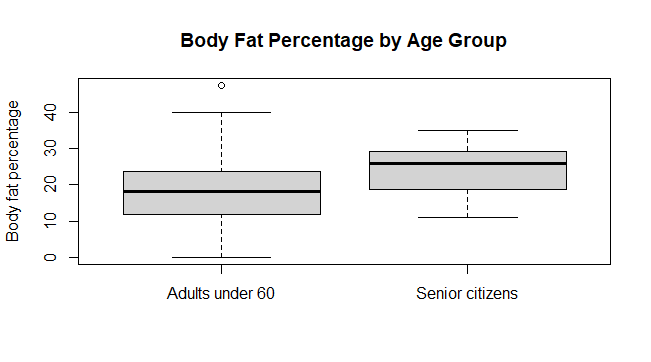
\includegraphics[width = 125mm]{agegroupbfpboxplot.png}
\caption{side-by-side box plot of body fat percentage by age group}
\label{side-by-side boxplot}
\end{figure}

\par The above figure tells us the sample mean of the senior citizen group is larger than the sample median for the younger adults. We can also see that the whiskers of the senior citizen's box plot are much smaller, suggesting a smaller sample variance than the younger adults. This plot gave provided a good idea of the underlying distributions, but a formal hypothesis test was required to make a definite decision. 

\par The younger group had a sample size of $n_1=214$ compare to the sample size of the older group of $n_2=36$.  Sample mean for the body fat percentage of the younger crowd was observed to be $\mu_{younger}=18.13598$ compare to the sample mean of the seniors whose observed sample mean was measured to be $\mu_{older}=24.36$. The younger sample standard deviation was measured to be $s_{younger}=8.25$ compared to $s_{older}=6.40$ of the seniors.  To formally test if the population means of the body fat percentage of the two groups were equivalent, or if they showed a significant difference from one another, the following null and alternate hypotheses are observed:
$\newline \newline$ $\centerline{$H_0:\mu_{younger}=\mu_{older},H_{\alpha}:\mu_{younger}\neq\mu_{older}.$} 
\newline \newline$
Given that both sample sizes are above 30, the central limit theorem could be applied to assume that both populations are normally distributed. This meant a Z-test could be performed even though the variance of the two samples is currently unknown. The z-test statistic for such an inference is as follows:

\begin{equation}
    Z=\frac{\bar{X}-\bar{Y}-(\mu_{younger}-\mu_{older})}{\sqrt{s_1^2/n_1+s_2^2/n_2}}.
\end{equation}

In the z-test statistic it is noted that $(\mu_{younger}-\mu_{older})=0$ under the observed null hypothesis. Plugging in the values above results in a z score of $Z=-5.1563$. This is a very low Z-value which tells us, based on the knowledge of the area under the standard normal curve, that the associated p-value will be very close to zero; this value can be approximated as $p=2.518*10^{-7}$. Given that the p-value is less than $\alpha=0.05$, null hypothesis can be rejected and the conclusion can be made that there is a significant difference in the mean body fat percentage of adults under 60 and senior citizens. 

\par Now that we know there is a significant difference between $\mu_{younger}$ and $\mu_{older}$, we can test to see which mean is larger. We initially suspected that $\mu_{younger}<\mu_{older}$ which would correspond to the hypotheses:
$\newline \newline$
$\centerline{$H_0:\mu_{younger}=\mu_{older}, H_{\alpha}:\mu_{younger}<\mu_{older}$}$
$\newline $
The test statistic for this test would be the same as for the previous test. Hence, $Z=-5.1563$ with a corresponding p-value of $p=1.259*10^{-7}$ which is half of the p-value of our first test. Since $1.259*10^{-7}<0.05$ we can reject the null hypothesis and conclude that the mean body fat percentage of seniors is higher than younger adults. 


\section*{Hypothesis 2}
The body fat data set was originally collected with the purpose of devising a better way to evaluate body fat percentage. Due to practical difficulties of existing methods, it was hypothesized that the variables measured in the data set could predict body fat, providing a more cost and time efficient alternative. To build an \textit{inferential} model and test whether or not this hypothesis holds, one can construct a multiple linear regression model, which accounts for multiple predictor variables influencing a response variable. The process of building such a model involves determining which predictor variables are statistically significant, and refining the model according to the assumptions of linear regression. The exact hypotheses take the form:


\begin{equation}
    H_0: \beta_i = 0, H_A: \beta_i \neq 0
\end{equation}


Where, in reference to table 1, $i$ ranges from 0 to 14, where $\beta_0$ is the intercept. The response variable is body fat percentage. The original data set contained a body density variable, however, this will not be used as a predictor variable. In fact, percentage body and body density are related through Siri's equation \cite{sciencedirect}:

\begin{equation}
    \% BF= (\frac{4.95}{Density} - 4.5) \times 100
\end{equation}

If the predictor variable has a statistically significant slope, then it should be included in the linear model, mathematically represented as:

\begin{equation}
    \boldsymbol{Y} = \boldsymbol{X\beta} + \boldsymbol{\epsilon}
\end{equation}

Where \textbf{Y} is the response variable vector, \textbf{X} is the predictor variable matrix, $\beta$ is the slope vector, and $\epsilon$ is the error. Inference on each $\beta_i$ is performed under a t-distribution with a t statistic:

\begin{equation}
    |t_i| = \frac{|\hat{\beta_i}|}{SE(\hat{\beta_i})} > t_{n - (k+1) , \alpha/2}
\end{equation}

Where $\hat{\beta_i}$ is the estimated slope of the i\textit{th} variable, $SE(\hat{\beta_i})$ is the standard error of each variable's slope, $n$ is the number of observations, $k$ is the number of variables, and $\alpha$ is the significance level. The inequality indicates the case of rejection, or that the variable has a statistically significant slope.

The F-test for the overall regression model assesses whether or not at least one predictor variable is related to the model. This test has hypotheses of the form:

\begin{equation}
    H_0: \beta_0 = ... = \beta_{14} = 0 , H_A: \beta_i \neq 0 \quad \textrm{for some i}
\end{equation}

Thus, if the multiple linear regression model has at least one accurate predictor variable, the F-test will reject $H_0$. Such as scenario is given by the following criterion:

\begin{equation}
    F = \frac{MSR}{MSE} > f_{k, n - (k+1), \alpha}
\end{equation}

Where $MSR$ is the mean square regression and is defined as $MSR = \frac{SSR}{1}$, and $MSE$ is the mean square error, defined by $MSE = \frac{SSE}{n-2}$. The last important parameter is the coefficient of multiple determination, which represents the percentage of variation in the response variable accounted for by regression on the predictor variables:

\begin{equation}
    r^2 = 1 - \frac{SSE}{SST}
\end{equation}
 
Where $SSE$ and $SST$, as referenced in the previous equation for the F-statistic, represent the error sum of squares and total sum of squares respectively.  In simple linear regression, the square root of the coefficient of determination yields the correlation coefficient, which measures the strength of the relation between the response variable and predictor variable. However, when many predictor variables are considered, the correlation coefficient becomes the \textit{multiple correlation coefficient}, and measures the same strength but between the response variable and the \textit{set} of predictor variables.

Now that the essential parameters and test statistics are briefed, the normality assumption must be checked to proceed with multiple linear regression. This is accomplished in the introduction.

The linear model command was used in R to output a multiple regression model. This command automatically performs inference on the $\beta_i$ values, and assigns a coefficient of multiple determination along with the overall F-statistic. Initially, the following model was used:

\begin{equation}
    y_{BF\%} = \beta_0 + \beta_1 x_1 + ... + \beta_{14} x_{14}
\end{equation}

Where, referring to the variable table, the integer subscript denotes to the corresponding variable. The regression output indicates which variables have a statistically significant slope, and is pictured in figure 3.

\begin{figure}[h]
\centering
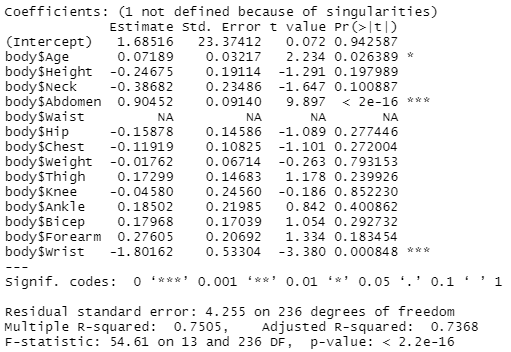
\includegraphics[width = 100mm]{model1_output.PNG}
\caption{Initial model's output in R Studio.}
\label{model1_output}
\end{figure}
We can check the assumptions of multiple linear regression with several plots, as seen in figure 4. The normal plot for residuals shows that the residuals are normally distributed. The residuals vs. fitted values plot checks for constant variance, and spread should be random around 0. The residuals vs. leverage plot should be random around 0 and leverage should be low, where leverage is how the fitted response behaves when the actual response changes. The standardized residuals vs fitted values plot is a standardized version of the residual plot. The output in figure 3 shows that approximately $75\%$ of the variation in $y$ is accounted for by the multiple regression model. Additionally, the p-value related to the F-statistic implies that there is a statistically significant linear relation with at least on the variables in the model. However, only three of of the fourteen variables are statistically significant at varying significance. This suggests that the model can be refined to be simpler, while retaining accuracy in the form of $r^2$. Typically, more variables will increase the multiple coefficient of determination, but convolutes the model and possibly introduce \textit{multicollinearity}, which invalidates the model results at high levels. Multicollinearity is a linear relation among several of the predictor variables. In other words, the correlation coefficient is non-trivial among mixed pairs of the predictor variables. This raises issues of linear dependence among the columns of \textbf{X} in equation (3), which must be invertible to perform inference on $\beta$. One technique of assessing this issue is calculating \textit{variance inflation factors}, which are the diagonal elements of the inverted correlation matrix \textbf{R}. Variance inflation factors greater than 10 usually give rise to problems in the model \cite{Tamhane}.

\begin{figure}
\begin{subfigure}{.45\textwidth}
  \centering
  % include first image
  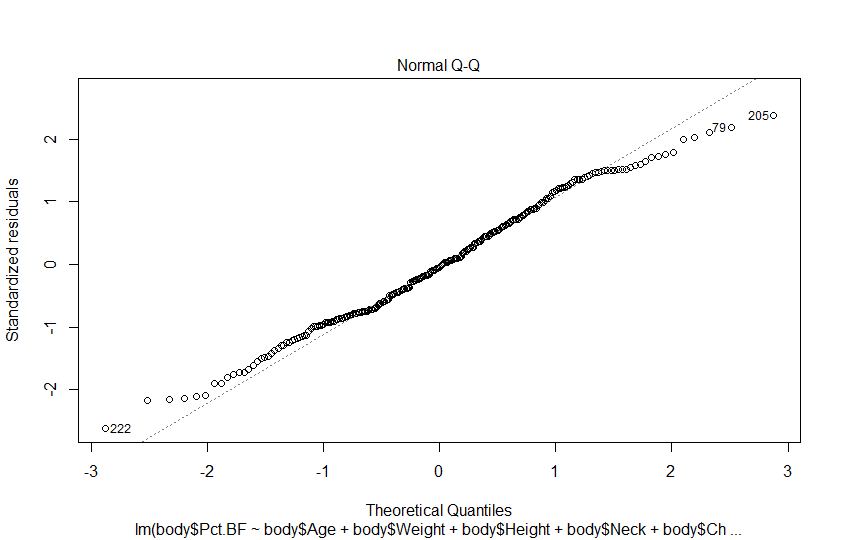
\includegraphics[width=.8\linewidth]{normqq1.png}  
  \caption{Normal plot for residuals}
  \label{fig:sub-first}
\end{subfigure}
\begin{subfigure}{.45\textwidth}
  \centering
  % include second image
  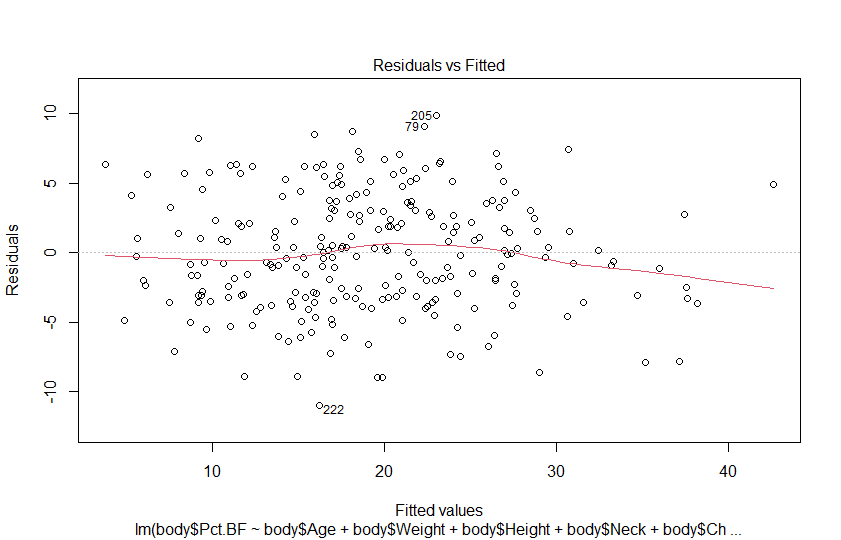
\includegraphics[width=.8\linewidth]{residvfit1.png}  
  \caption{Residuals vs. fitted values}
  \label{fig:sub-second}
\end{subfigure}

\newline

\begin{subfigure}{.45\textwidth}
  \centering
  % include third image
  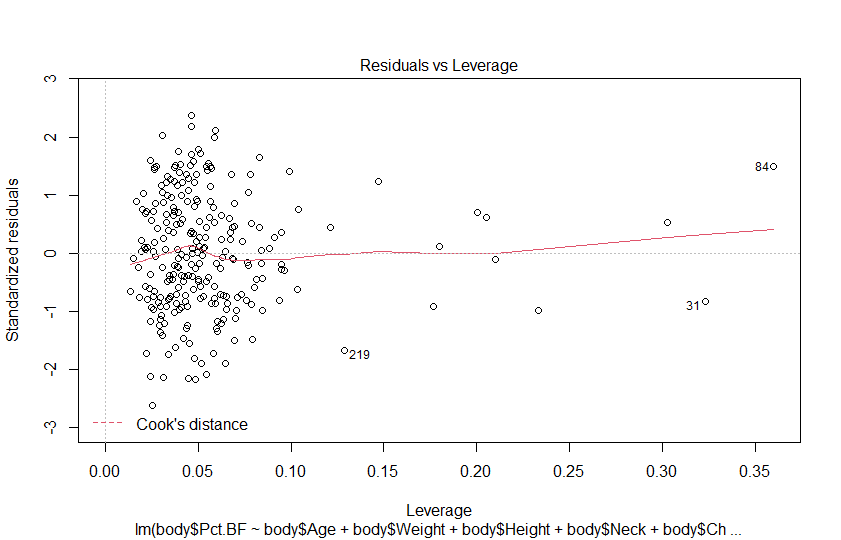
\includegraphics[width=.8\linewidth]{residvlev1.png}  
  \caption{Residuals vs. leverage}
  \label{fig:sub-third}
\end{subfigure}
\begin{subfigure}{.45\textwidth}
  \centering
  % include fourth image
  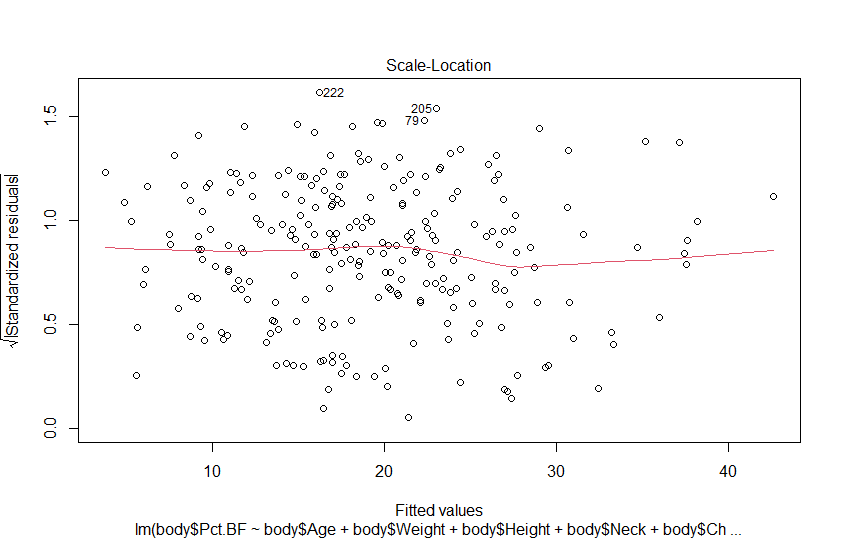
\includegraphics[width=.8\linewidth]{scaleloc1.png}  
  \caption{Standardized residuals vs fitted values (scale location)}
  \label{fig:sub-fourth}
\end{subfigure}
\caption{Plots to check assumptions for initial model}
\label{fig:fig}
\end{figure}

It should be noted that for all additional analysis, the waist variable was removed from the model. This is due to its strong linear dependence with at least one the other predictor variables, leading to errors during regression. This behavior is confirmed with the alias function in R.

After removing the waist variable, variance inflation factors were computed for each predictor variable. The variables with VIFs greater than 10 are: Weight, Chest, Hip, and Abdomen. Unfortunately, Abdomen is the strongest predictor of percentage body fat according to the initial model output, so it would be unfavorable to remove this variable form the model. Perhaps, at this point, it would be best to remove all statistically insignificant variables, and address multicollinearity afterward. It is possible that abdomen is linearly dependent with one of the insignificant variables, so removing them would cause no issues with the model's accuracy and improve abdomen's VIF.  

The stepwise regression variable choosing algorithm was used to select statistically significant variables and refine the model. This algorithm runs partial F-tests on successive subsets of the variables, until the whole list of variables has been iterated through. It eliminates variables if their partial F-statistics do not exceed some criterion \cite{Tamhane}. The result is a refined model, which will have a similar coefficient of determination but fewer variables, hopefully mitigating multicollinearity and simplifying the practical components of using the model. In a clinical setting, fewer body dimensions would be required to get the same prediction of percentage body fat. The results of stepwise linear regression can be seen in figure 5.

\begin{figure}[h]
\centering
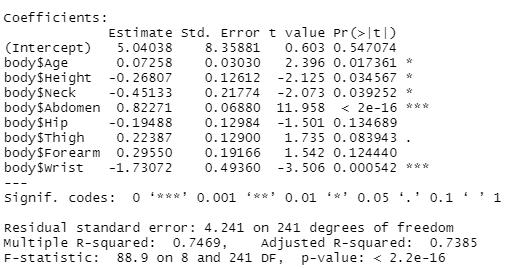
\includegraphics[width = 100mm]{stepmodel_output.PNG}
\caption{Stepwise linear regression algorithm applied to the original model.}
\label{stepmodel}
\end{figure}

This algorithm was applied using the stepAIC function in R. Backward stepwise regression was used, which eliminates variables from the original set. This function is slightly different than the one explained above, in that it eliminates variables based on the Aikake Information Criterion as opposed to the partial F-statistic. As displayed, the algorithm eliminated the chest, weight, and bicep variables. The waist variable was not included in the algorithm input. 

\begin{figure}[h]
\centering
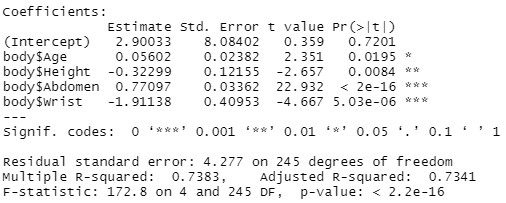
\includegraphics[width = 100mm]{stepmodel_reducedoutput.PNG}
\caption{Final multiple linear regression model for percentage body fat response variable.}
\label{stepmodel_reduced}
\end{figure}

The output shows that approximately $74.7\%$ of the variation in y is accounted for by the model. This is a drop of merely $0.4\%$ when compared to the original model. By reducing the number of variables, not only is the model simplified, but multicollinearity risk has been reduced. Re-running VIF tests yields only one value close to 10, that of the Hip variable. Additionally, if a significance level of 0.05 is used, the forearm and thigh variables can be eliminated as well. Removing these outputs a  slightly lower $r^2$ of 0.7404. This model now indicates that the neck variable is insignificant, so it is eliminated too. The age, height, abdomen, and wrist variables remain, with a coefficient of multiple determination $r^2$ of 0.7383. 

\begin{figure}
\begin{subfigure}{.45\textwidth}
  \centering
  % include first image
  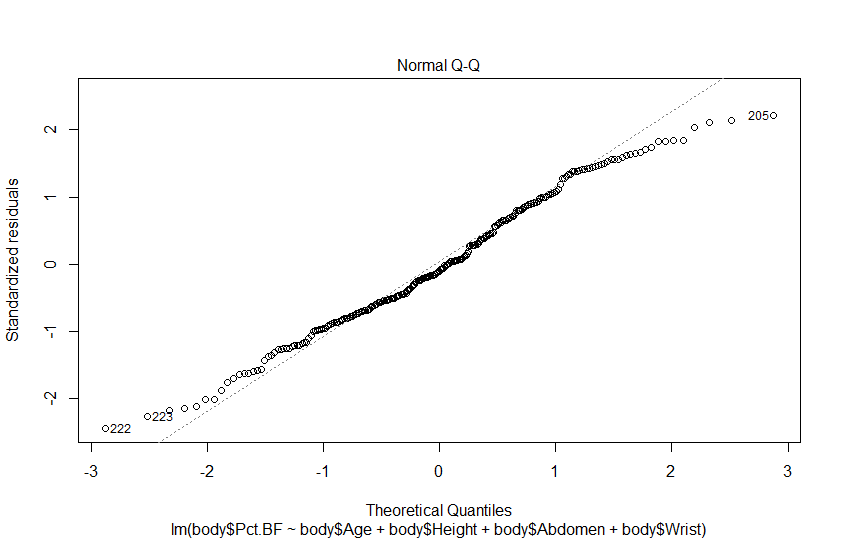
\includegraphics[width=.8\linewidth]{normqq2.png}  
  \caption{Normal plot for residuals}
  \label{fig:sub-first}
\end{subfigure}
\begin{subfigure}{.45\textwidth}
  \centering
  % include second image
  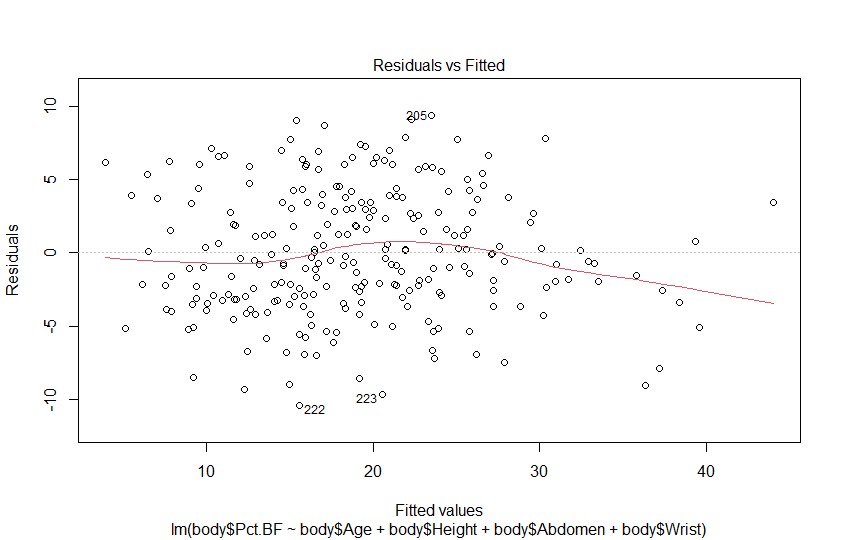
\includegraphics[width=.8\linewidth]{residvfit2.png}  
  \caption{Residuals vs. fitted values}
  \label{fig:sub-second}
\end{subfigure}

\newline

\begin{subfigure}{.45\textwidth}
  \centering
  % include third image
  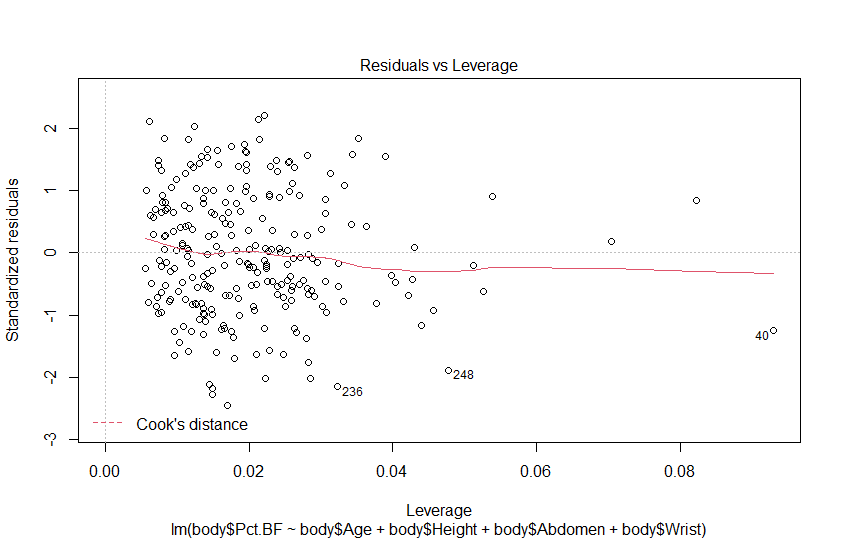
\includegraphics[width=.8\linewidth]{residvlev2.png}  
  \caption{Residuals vs. leverage}
  \label{fig:sub-third}
\end{subfigure}
\begin{subfigure}{.45\textwidth}
  \centering
  % include fourth image
  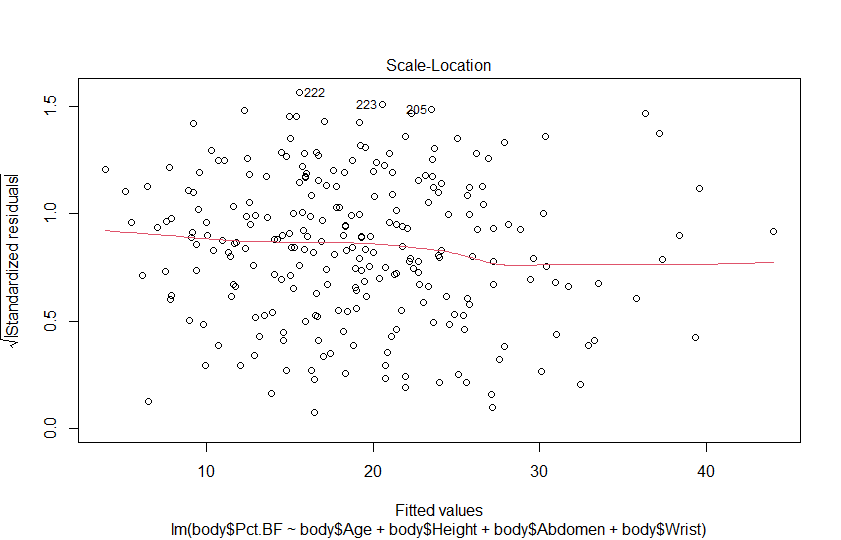
\includegraphics[width=.8\linewidth]{scaleloc2.png}
  
  \caption{Standardized residuals vs fitted values (scale location)}
  \label{fig:sub-fourth}
\end{subfigure}
\caption{Plots to check assumptions for refined model}
\label{fig:fig2}
\end{figure}

This result, in a clinical setting, allows for the measurement of only three body dimensions with a reduction of only $1.22\%$ in the amount of variation in y accounted for by the model. The results can be seen in figure 6.



All variables have statistically significant slope estimations, and the VIF for each variable is below 2, which suggests minimal multicollinearity. The assumptions for this model can be checked with a sequence of plots as seen in figure 7. It should be noted that the goal of this particular regression was to determine if bodily dimensions and age could solely predict a man's percentage body fat. 



\subsection*{Random Removal of Data}

Random removal of data from the data set simulates having a smaller data set. Theoretically, random omission of data will not have a systematic pattern, and will not favor any phenomena or trends in the data. However, fewer observations will affect the statistical outcome of the experiment, and coincidentally, it may remove some outliers from the set, having a significant impact on results. 

\begin{figure}[h]
\centering
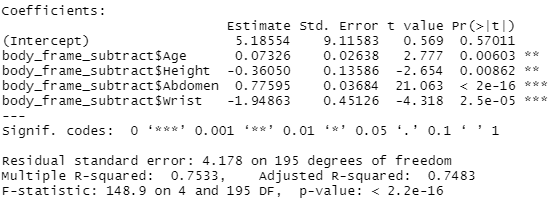
\includegraphics[width = 100mm]{reduced_results.PNG}
\caption{Multiple linear regression model on a randomly omitted data set.}
\label{stepmodel_reduced_omitted}
\end{figure}



The data was reduced by $20\%$. This was done by generating an array of 50 random numbers and subtracting that array from the data table stored in R. This removes the corresponding rows, and changes the total data set to 200 observations as opposed to 250.


\begin{figure}
\begin{subfigure}{.45\textwidth}
  \centering
  % include first image
  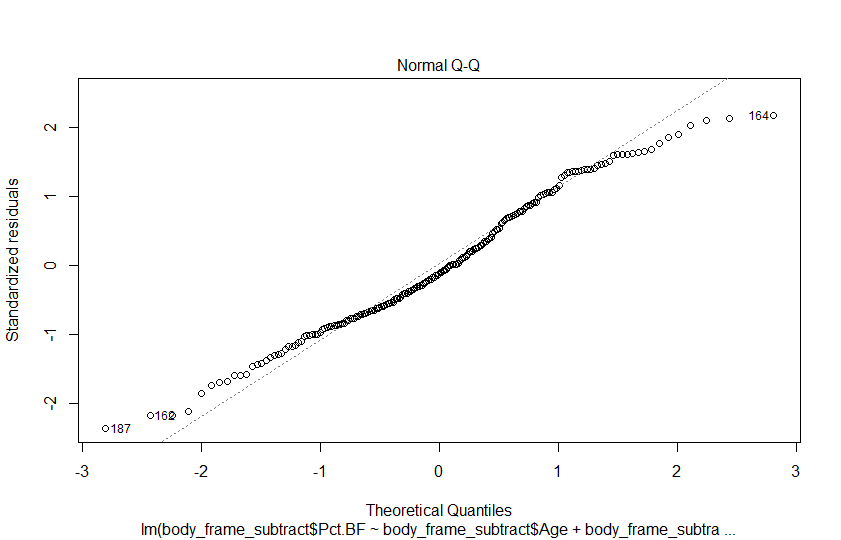
\includegraphics[width=.8\linewidth]{normqq3.png}  
  \caption{Normal plot for residuals}
  \label{fig:sub-first}
\end{subfigure}
\begin{subfigure}{.45\textwidth}
  \centering
  % include second image
  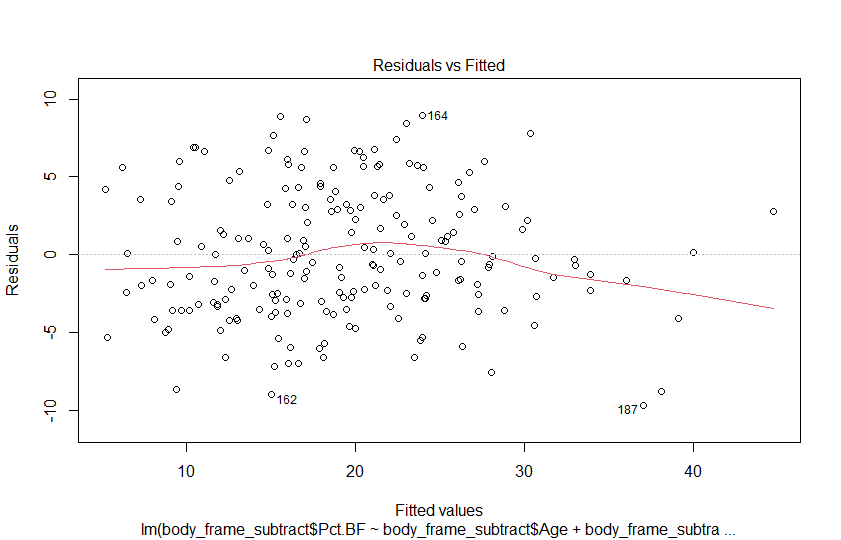
\includegraphics[width=.8\linewidth]{residvfit3.png}  
  \caption{Residuals vs. fitted values}
  \label{fig:sub-second}
\end{subfigure}

\newline

\begin{subfigure}{.45\textwidth}
  \centering
  % include third image
  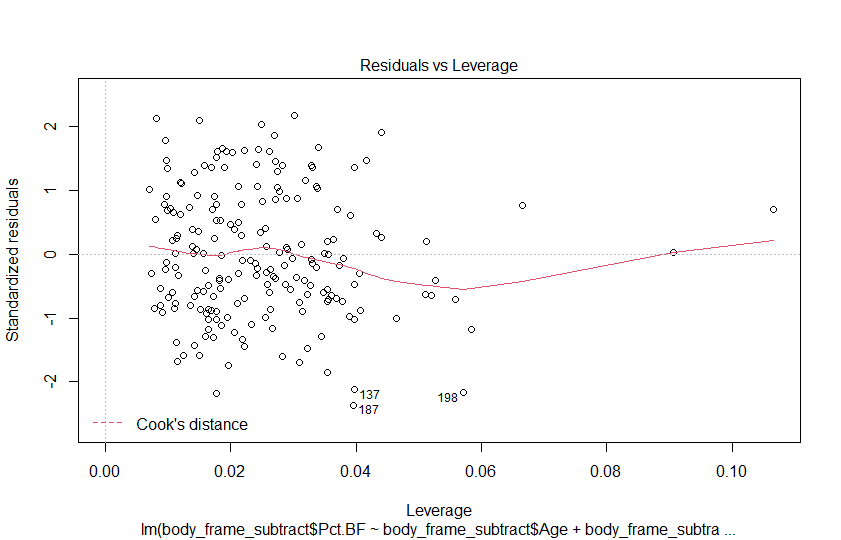
\includegraphics[width=.8\linewidth]{residvlev3.png}  
  \caption{Residuals vs. leverage}
  \label{fig:sub-third}
\end{subfigure}
\begin{subfigure}{.45\textwidth}
  \centering
  % include fourth image
  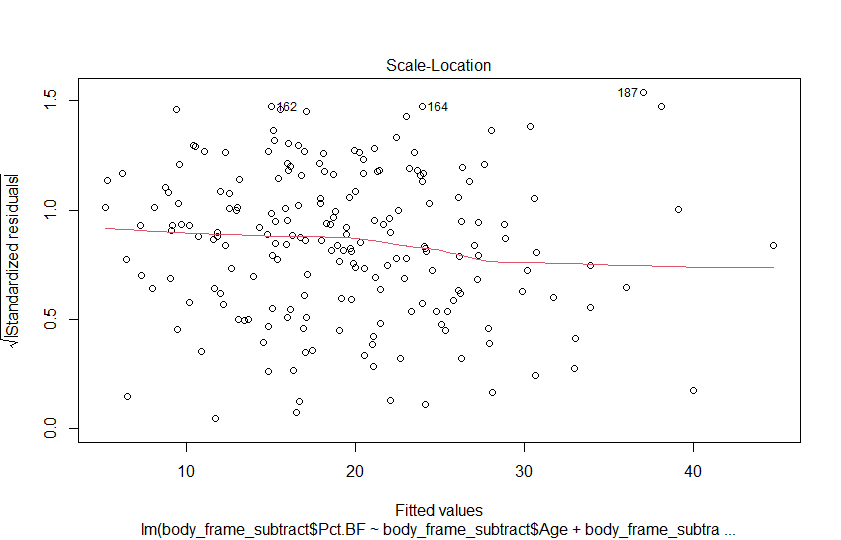
\includegraphics[width=.8\linewidth]{scaleloc3.png}
  
  \caption{Standardized residuals vs fitted values (scale location)}
  \label{fig:sub-fourth}
\end{subfigure}
\caption{Plots to check assumptions for randomly removed data model}
\label{fig:fig}
\end{figure}

After performing a regression analysis identical to the full data set, the results in the corresponding figure were obtained.

Figure 9 depicts the assumption plots. Each factor has a statistically significant slope at a 0.05 significance level. Additionally, the VIF for each variable is below two. Even after removing the same amount of variables, the coefficient of multiple determination in this case is $r^2 = 0.7533$, approximately 0.015 higher than the original model's $r^2$ value. The plots for this results can be seen in the corresponding figure. This increase in the coefficient of multiple determination can be explained by the possible removal of outliers. Equation (8) shows that decreasing $SSE$, the error sum of squares, will increase $r^2$. $SSE$ measures the overall goodness of fit, or how much the response values differ from the model. So if outliers from the model were randomly removed, this can increase the accuracy of the model\cite{Tamhane}.























\subsection*{Non-Ignorable Missing Data}

Dealing with data that is missing for a specific reason requires more care than if the data was missing completely at random. If the data was missing because someone just forgot to put a few values into the dataset, we could simply delete this observations from the data without worrying about bias. Our option for dealing with non-ignorable missing data would be to impute the missing values using any of a number of techniques.

\par Suppose younger men with a large weight and high body fat percentage were too self conscious to complete some of the body measurements. Deleting these observations from the data would make it seem as though seniors had a higher body fat percentage and skew the data. Our other option would be to use imputation to replace these values. Some less rigorous methods of imputation include hot-deck and cold-deck. For the cold-deck method, we would just look at similar datasets, take the necessary data where needed, and plug it into our original dataset where the values are missing. The hot-deck  method would include ordering our data in some way, possibly from smallest value to largest, and then filling in the missing value with the previous index's data. More concretely, if our $jth$ variable had a missing value in index $ith$ observation, we would fill it with the data from the $(i-1)th$ observation. Neither of these methods are very rigorous and introduce a large amount of bias. There are other methods which yield much better results. \cite{statfi}

\par We can also use linear regression to predict these missing values. There are two methods, deterministic and stochastic regression imputation. The problem with deterministic regression is that the replacement values fit the data too well, the value would sit directly on the hyperplane. The real value would have some variation. Stochastic regression imputation overcomes this problem by adding a normally distributed random error. This helps to further reduce the bias.\cite{Columbia}

\par There are many methods for imputation but stochastic imputation would have been our go-to method.


\printbibliography[title={References}]

\end{document}
